\chapter{Hash Tables}
\label{ch:hashing}

\newcommand{\lecnum}{12}
%\newcommand{\lectitle}{Hashing Tables}
\newcommand{\lecturer}{Frank Pfenning, Rob Simmons}

\chapterTAGS{amortized-cost, average-cost, complexity, dictionary, hashing, linked-list, randomness}
\maketitle

\begin{preamble}
\noindent
\emph{Dictionaries}, also called \emph{associative arrays} as well as
\emph{maps}, are data structures that are similar to arrays but are
not indexed by integers, but by possibly other forms of data such as
strings.  One popular data structure for the implementation of
dictionaries are \emph{hash tables}.  To analyze the asymptotic
efficiency of hash tables we have to explore a new point of view, that
of \emph{average case complexity}.  Another computational thinking
concept that we revisit is \emph{randomness}.  In order for hash
tables to work efficiently in practice we need hash functions whose
behavior is predictable (deterministic) but has some aspects of
randomness.
\end{preamble}

\begin{gram}[Learning Goals]
Relating to our learning goals, we have
\begin{description}

\item[Computational Thinking: ]%
  We consider the importance of \emph{randomness} in algorithms, and also
  discuss \emph{average case analysis}, which is how we can argue that hash
  tables have acceptable performance.

\item[Algorithms and Data Structures: ]%
  We describe a \emph{linear congruential generator}, which is a certain kind
  of \emph{pseudorandom number generator}. We also discuss hashtables and
  their implementation with \emph{separate chaining} (an array of linked
  lists).

\item[Programming: ]%
  We review the implementation of the \lstinline'rand' library in C0.
\end{description}
\end{gram}


\section{Dictionaries, Associative Arrays, or Maps}
\label{sec:hashing:mappings}
\TAGS{dictionary}

An array $A$ can be seen as a mapping $i \mapsto v$ that associates a
value $v$ (which we denote $A[i]$) with every index $i$ in the range
$\lbrack 0, \backslash\mathit{length}(A))$.  It is finitary, because its
domain, and therefore also its range, is finite.  There are many
situations when we want to index elements differently than just by
contiguous integers starting at 0.  Common examples are strings (for
dictionaries, phone books, menus, database records), or structs (for
dates, or names together with other identifying information).  Such
generalized arrays are called \emph{dictionaries} or \emph{associative
  arrays} or \emph{maps}.  These situations are so common that
dictionaries are primitive in some languages such as PHP, Python, or
Perl and perhaps account for some of the popularity of these
languages.  In many applications, dictionaries are implemented as hash
tables because of their performance characteristics.  We will develop
them incrementally to understand the motivation underlying their
design.


\section{Keys, Entries and Values}
\label{sec:hashing:keys_entries_values}
\TAGS{dictionary}

In many applications requiring dictionaries, we are storing complex
data and want to access them by a \emph{key} which is derived from the
data.  For example, the key might be a student id (a string) and the
data might be this student's record, which may itself record her
grades in a dictionary whose keys are the name of each assignment or
exam and the data is a score.  We make the assumption that keys are
unique in the sense that in a dictionary there is at most one data
item associated with a given key --- here no two students have the
same id and no two assignments have the same name.

The data item associated to a key in a dictionary is variously called
an \emph{entry} or a \emph{value}.  We tend to use the word entry when
the key is part of the data (like a student record) and the word
value when it is not (for example, the average temperature of each day
of the year).

We can think of built-in C0 arrays as dictionaries having a set number
of keys: a C0 array of length 3 has three keys \lstinline'0',
\lstinline'1', and \lstinline'2'.  Our implementation of unbounded
arrays allowed us to add a specific new key, \lstinline'3', to such an
array.  We do want to be able to add new keys to the dictionary.  We
also want our dictionaries to allow us to have more interesting keys
(like strings, or non-sequential integers) while keeping the property
that there is a unique entry for each valid key.


\section{Chains}
\label{sec:hashing:chaining}
\TAGS{complexity, dictionary, linked-list}

A first idea to explore is to implement the dictionary as a linked
list, called a \emph{chain}.  If we have a key $k$ and look for it in
the chain, we just traverse it, compute the intrinsic key for each
data entry, and compare it with $k$.  If they are equal, we have found
our entry, if not we continue the search.  If we reach the end of the
chain and do not find an entry with key $k$, then no entry with the
given key exists.  If we keep the chain unsorted this gives us $O(n)$
worst case complexity for finding a key in a chain of length $n$,
assuming that computing and comparing keys is constant time.

Given what we have seen so far in our search data structures, this
seems very poor behavior, but if we know our data collections will
always be small, it may in fact be reasonable on occasion.

Can we do better?  One idea goes back to binary search.  If keys are
ordered we may be able to arrange the elements in an array or in the
form of a tree and then cut the search space roughly in half every
time we make a comparison.  Designing such data structures is a rich
and interesting subject, but the best we can hope for with this
approach is $O(\log n)$, where $n$ is the number of entries.  We have
seen that this function grows very slowly, so this is quite a
practical approach.

Nevertheless, the challenge arises if we can do better than $O(\log
n)$, say, constant time $O(1)$ to find an entry with a given key.  We
know that it can done be for arrays, indexed by integers, which allow
constant-time access.  Can we also do it, for example, for strings?


\section{Hashing}
\label{sec:hashing:hashing}
\TAGS{dictionary, hashing}

The first idea behind hash tables is to exploit the efficiency of
arrays.  So: to map a key to an entry, we first map a key to an
integer and then use the integer to index an array $A$.  The first map
is called a \emph{hash function}.  We write it as $\mathrm{hash}(\_)$.
Given a key $k$, our access could then simply be
$A[\mathrm{hash}(k)]$.

There is an immediate problem with this approach: there are
$2^{31}$ positive integers, so we would need a huge array, negating
any possible performance advantages.  But even if we were willing to
allocate such a huge array, there are many more strings than
\lstinline'int''s so there cannot be any hash function that always gives us
different \lstinline'int''s for different strings.

The solution is to allocate an array of smaller size, say $m$, and then look
up the result of the hash function modulo $m$, for example,
$A[\mathrm{hash}(k) \% m]$.  This idea has an obvious problem: it is
inevitable that multiple strings will map to the same array index.  For
example, if the array has size $m$ then if we have more then $m$ elements, at
least two must map to the same index --- this simple observation is an
instance of what is known as the \emph{pigeonhole principle}.  In practice,
this will happen much sooner than this.

If a hash function maps two keys to the same integer value (modulo
$m$), we say we have a \emph{collision}.  In general, we would like to
avoid collisions, because some additional operations will be required
to deal with them, slowing down search and taking more space.  We
analyze the cost of collisions more below.


\section{Separate Chaining}
\label{sec:hashing:separate_chaining}
\TAGS{hashing, linked-list}

How do we deal with collisions of hash values?  The simplest is a
technique called \emph{separate chaining}.  Assume we have
$\mathrm{hash}(k_1)\%m = i = \mathrm{hash}(k_2)\%m$, where $k_1$ and
$k_2$ are the distinct keys for two data entries $e_1$ and $e_2$ we
want to store in the table.  In this case we just arrange $e_1$ and
$e_2$ into a chain (implemented as a linked list) and store this list
in $A[i]$.

In general, each element $A[i]$ in the array will either be
\lstinline'NULL' or a chain of entries.  All of these must have the same
hash value for their key (modulo $m$), namely $i$.  As an exercise,
you might consider other data structures here instead of chains and
weigh their merits: how about sorted lists?  Or queues?  Or
doubly-linked lists?  Or another hash table?

We stick with chains because they are simple and fast, provided the
chains don't become too long.  This technique is called
\emph{separate} chaining because the chains are stored separately, not
directly in the array.  Another technique, which we will not discuss
at length, is \emph{linear probing} where we continue by searching
(linearly) for an unused spot in the array itself, starting from the
place where the hash function put us.

Under separate chaining, a snapshot of a hash table might
look something like this picture.
\begin{center}
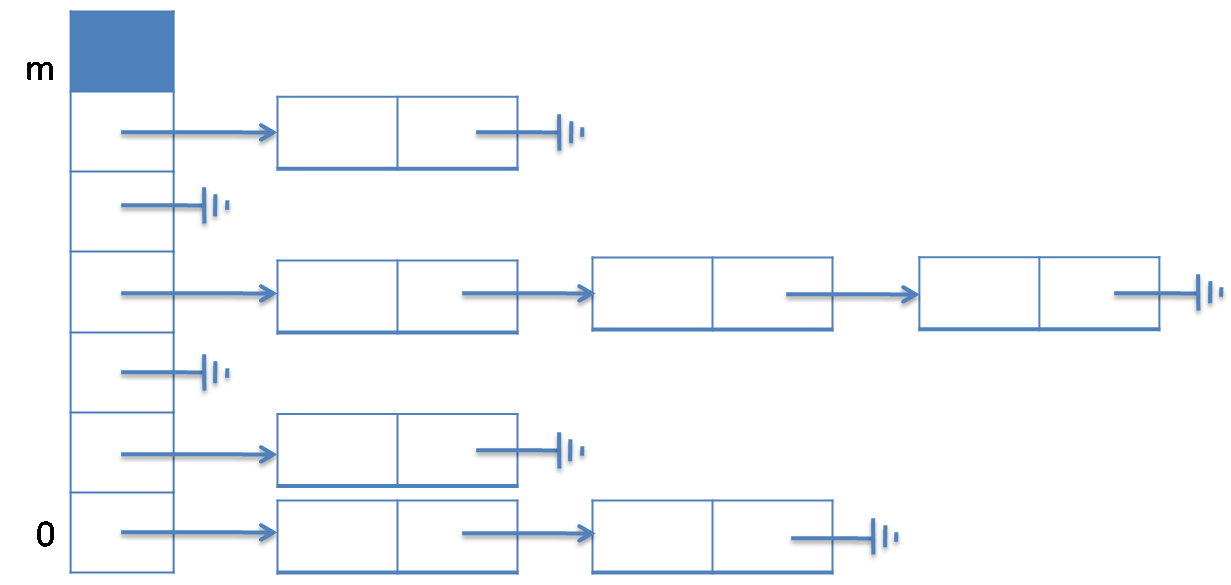
\includegraphics[width=0.9\textwidth]{img/hashtable1.png}
\end{center}


\section{Average Case Analysis}
\label{sec:hashing:average_case}
\TAGS{amortized-cost, complexity, hashing}

How long do we expect the chains to be on average?  For a
total number $n$ of entries in a table of size $m$, it
is $n/m$.  This important number is also called the \emph{load
factor} of the hash table.  How long does it take to search
for an entry with key $k$?  We follow these steps:
\begin{enumerate}
\item Compute $i = \mathrm{hash}(k) \% m$.  This will be $O(1)$
  (constant time), assuming it takes constant time to compute
  the hash function.
\item Go to $A[i]$, which again is constant time $O(1)$.
\item Search the chain starting at $A[i]$ for an
  element whose key matches $k$.  We will analyze
  this next.
\end{enumerate}
The complexity of the last step depends on the length of the chain.
In the \emph{worst case} it could be $O(n)$, because all $n$ elements
could be stored in one chain.  This worst case could arise if we
allocated a very small array (say, $m = 1$), or because the hash
function maps all input strings to the same table index $i$, or just
out of sheer bad luck.

Ideally, all the chains would be approximately the same length, namely
$n/m$.  Then for a fixed load factor such as $n/m = \alpha = 2$ we
would take on average 2 steps to go down the chain and find $k$.  In
general, as long as we don't let the load factor become too large, the
\emph{average} time should be $O(1)$.

If the load factor does become too large, we could dynamically adapt the size
of the array, like in an unbounded array.  As for unbounded arrays, it is
beneficial to double the size of the hash table when the load factor becomes
too high, or possibly halve it if the size becomes too small.  Analyzing these
factors is a task for amortized analysis, just as for unbounded arrays.


\section{Randomness}
\label{sec:hashing:randomness}
\TAGS{average-cost, complexity, hashing, randomness}

The average case analysis relies on the fact that the hash values of
the key are relatively evenly distributed.  This can be restated as
saying that the probability that each key maps to an array index $i$
should be about the same, namely $1/m$.  In order to avoid
systematically creating collisions, small changes in the input string
should result in unpredictable change in the output hash value that is
uniformly distributed over the range of C0 integers.  We can achieve
this with a \emph{pseudorandom number generator} (PRNG).  A
pseudorandom number generator is just a function that takes one number
and obtains another in a way that is both unpredictable and easy to
calculate.  The C0 \lstinline'rand' library is a pseudorandom number
generator with a fairly simple interface:
\begin{lstlisting}[language={[C0]C}]
/* library file rand.h0 */
typedef struct rand* rand_t;
rand_t init_rand (int seed);
int rand(rand_t gen);
\end{lstlisting}
One can generate a random number generator (type \lstinline'rand_t') by
initializing it with an arbitrary seed.  Then we can generate a
sequence of random numbers by repeatedly calling \lstinline'rand' on such a
generator.

The \lstinline'rand' library in C0 is implemented as a \emph{linear
  congruential generator}. A linear congruential generator takes a number $x$
and finds the next number by calculating $(a \times x) + c$ modulo $d$, a
number that is used as the next $x$. In C0, it's easiest to say that $d$ is
just $2^{32}$, since addition and multiplication in C0 are already defined
modulo $2^{32}$. The trick is finding a good multiplier $a$ and summand $c$.

If we were using 4-bit numbers (from $-8$ to $7$ where multiplication
and addition are modulo 16) then we could set $a$ to 5 and $c$ to 7
and our pseudorandom number generator would generate the following
series of numbers:
\begin{align*}
0 & \rightarrow
7 \rightarrow
(-6) \rightarrow
(-7) \rightarrow
4 \rightarrow
(-5) \rightarrow
(-2) \rightarrow
\\
 & -3 \rightarrow
(-8) \rightarrow
(-1) \rightarrow
1 \rightarrow
(-4) \rightarrow
3 \rightarrow
6 \rightarrow
5 \rightarrow
0 \rightarrow \ldots
\end{align*}

The PRNG used in C0's library sets $a$ to $1664525$ and
$c$ to $1013904223$ and generates the following series of numbers starting
from $0$:
$$
0 \rightarrow
1013904223 \rightarrow
1196435762 \rightarrow
(-775096599) \rightarrow
(-1426500812) \rightarrow \ldots
$$
This kind of generator is fine for random testing or (indeed) the
basis for a hashing function, but the results are too predictable to
use it for cryptographic purposes such as encrypting a message.  In
particular, a linear congruential generator will sometimes have
repeating patterns in the lower bits.  If one wants numbers from a
small range it is better to use the higher bits of the generated
results rather than just applying the modulus operation.

It is important to realize that these numbers just \emph{look} random,
they aren't really random.  In particular, we can reproduce the exact
same sequence if we give it the exact same seed.  This property is
important for both testing purposes and for hashing. If we discover a
bug during testing with pseudorandom numbers, we want to be able to
reliably reproduce it, and whenever we hash the same key using
pseudorandom numbers, we need to be sure we will get the
same result.

\begin{lstlisting}[language={[C0]C}, numbers=left]
/* library file rand.c0 */
struct rand {
  int seed;
};

rand_t init_rand (int seed) {
  rand_t gen = alloc(struct rand);
  gen->seed = seed;
  return gen;
}

int rand(rand_t gen) {
  gen->seed = gen->seed * 1664525 + 1013904223;
  return gen->seed;
}
\end{lstlisting}

Observe that some choices of the numbers $a$ and $c$ would be
terrible.  For example, if we were to work with 4-bit numbers, so that
$d = 16$, choosing $a= 0$ would mean that our ``pseudo-random''
generator always returns $c$.  Were we to choose $a = c = 4$, it would
only return values among $-8$, $-4$, 0, and 4.  In general, we want,
at a minimum, that the factor $c$ and the modulus $d$ be
\emph{relatively prime}, i.e., that their greatest common divisor be
1.

\clearpage
\section{Exercises}
\label{sec:hashing:exercises}

 \begin{exercise}
   What happens when you replace the data structure for separate
   chaining by something other than a linked list? Discuss the changes
   and identify benefits and disadvantages when using a sorted list, a
   queue, a doubly-linked list, or another hash table for separate
   chaining.
 \end{exercise}

 \begin{exercise}
   Consider the situation of writing a hash function for strings of length
   two, that only use the characters \lstinline!'A'! to \lstinline!'Z'!.
   There are $26 \times 26 = 676$ different such strings. You were hoping to
   get away with implementing a hash table without collisions, since you are
   only using 79 out of those 676 two-letter words.  But you still see
   collisions most of the time.  Look up the \emph{birthday paradox} and use
   it to explain this phenomenon.
 \end{exercise}

% \clearpage
% \bibliographystyle{alpha}
% \bibliography{modal}

% \cleardoublepage
